\documentclass[12pt,letterpaper]{article}

% just for the example
\usepackage{lipsum}
% Set margins to 1.5in
\usepackage[margin=1.5in]{geometry}
\usepackage[toc,page]{appendix}

% for graphics
\usepackage{graphicx}
\graphicspath{{./figures/m2/}}

% for crimson text
\usepackage{crimson}
\usepackage[T1]{fontenc}
\usepackage{url}

% setup parameter indentation
\setlength{\parindent}{0pt}
\setlength{\parskip}{6pt}

% for 1.15 spacing between text
\renewcommand{\baselinestretch}{1.15}

% For defining spacing between headers
\usepackage{titlesec}
% Level 1
\titleformat{\section}
  {\normalfont\fontsize{18}{0}\bfseries}{\thesection}{1em}{}
% Level 2
\titleformat{\subsection}
  {\normalfont\fontsize{14}{0}\bfseries}{\thesection}{1em}{}
% Level 3
\titleformat{\subsubsection}
  {\normalfont\fontsize{12}{0}\bfseries}{\thesection}{1em}{}
% Level 4
\titleformat{\paragraph}
  {\normalfont\fontsize{12}{0}\bfseries\itshape}{\theparagraph}{1em}{}
% Level 5
\titleformat{\subparagraph}
  {\normalfont\fontsize{12}{0}\itshape}{\theparagraph}{1em}{}
% Level 6
\makeatletter
\newcounter{subsubparagraph}[subparagraph]
\renewcommand\thesubsubparagraph{%
  \thesubparagraph.\@arabic\c@subsubparagraph}
\newcommand\subsubparagraph{%
  \@startsection{subsubparagraph}    % counter
    {6}                              % level
    {\parindent}                     % indent
    {12pt} % beforeskip
    {6pt}                           % afterskip
    {\normalfont\fontsize{12}{0}}}
\newcommand\l@subsubparagraph{\@dottedtocline{6}{10em}{5em}}
\newcommand{\subsubparagraphmark}[1]{}
\makeatother
\titlespacing*{\section}{0pt}{12pt}{6pt}
\titlespacing*{\subsection}{0pt}{12pt}{6pt}
\titlespacing*{\subsubsection}{0pt}{12pt}{6pt}
\titlespacing*{\paragraph}{0pt}{12pt}{6pt}
\titlespacing*{\subparagraph}{0pt}{12pt}{6pt}
\titlespacing*{\subsubparagraph}{0pt}{12pt}{6pt}

% Set caption to correct size and location
\usepackage[tableposition=top, figureposition=bottom, font=footnotesize, labelfont=bf]{caption}

% set page number location
\usepackage{fancyhdr}
\fancyhf{} % clear all header and footers
\renewcommand{\headrulewidth}{0pt} % remove the header rule
\rhead{\thepage}
\pagestyle{fancy}

% Overwrite Title
\makeatletter
\renewcommand{\maketitle}{\bgroup
   \begin{center}
   \textbf{{\fontsize{18pt}{20}\selectfont \@title}}\\
   \vspace{10pt}
   {\fontsize{12pt}{0}\selectfont \@author} 
   \end{center}
}
\makeatother

% Used for Tables and Figures
\usepackage{float}

% For using lists
\usepackage{enumitem}

% For using APA Citation format
\usepackage{apacite}

% Custom Quote
\newenvironment{myquote}[1]%
  {\list{}{\leftmargin=#1\rightmargin=#1}\item[]}%
  {\endlist}
  
% Create Abstract 
\renewenvironment{abstract}
{\vspace*{-.5in}\fontsize{12pt}{12}\begin{myquote}{.5in}
\noindent \par{\bfseries \abstractname.}}
{\medskip\noindent
\end{myquote}
}

\begin{document}

% Set Title, Author, and email
\title{Assignment M2}
\author{Snejana Shegheva \\ sshegheva3@gatech.edu}

\maketitle
\thispagestyle{fancy}

\begin{abstract}
Mapping data from one form to another for its ease-of-use is at the core of the \textit{Extract, Transform and Load} process \cite{wiki:etl}. There exist many tools that can accomplish the task of creating and maintaining a data warehouse. However, sometimes it is advantageous to have a custom solution that allows a user to interact with the data directly during some or all of the ETL phases. In this project, we analyze an internal interface of a \textit{transform} task that prepares the data for use in a personalized recommendation system powered by Artificial Intelligence engines. Our main goal is to assess all the weak areas of the existing interface to provide recommendations for alternative models that simplify the user interaction without assuming any pre-existing knowledge of the tool.
\end{abstract}

\subsection*{Needfinding Plan 1 - Participant Observation}
In the Participant Observation approach, we experience the task ourselves and record both, the steps performed and their outcomes to analyze the effectiveness and usability of the interface for the given task. 

To get started with a transformation task, I first need to get input data. For this project, I chose to retrieve data from the website \textit{http://arxiv.org} that provides an open access to papers in Physics, Mathematics, Computer Science, and other fields. After loading the data into the system and extracting 30 fields, such as \textit{authors}, \textit{title}, \textit{summary}, \textit{published}, etc., I was presented with a view that allows seeing each property's metadata - \textit{id}, \textit{name}, \textit{data type}, and an option to \textit{Edit} the property. Pressing the \textit{Edit} button enters the interface portion that deals with transformation task for a chosen property.    

\textbf{Goal}: From a data property, \textit{published}, that has a format \textit{dd-mm-yy}, I wish to extract the \textit{year} portion only so I can possibly use it as a feature in the platform algorithms. 

\textbf{Task}: Find the original property \textit{published}, find a transformation that keeps only the last two digits, and store the result in a new property \textit{year}.

After briefly looking at the list of available transformation functions, the closest candidate I found was \textit{RegexTransformer}, an internal wrapper over the regular expression language \cite{wiki:regex}. This prompted a new \textbf{subtask}: generate a correct expression that finds the last two digits in a string. Trial, error, and Google eventually led me to an expression "{\textbackslash{d}\{2\}\$}" that provided the output I was expecting. Hitting \textit{Save} button saves my preference and applies the transformation to the entire dataset.

\textbf{Observations}:

1) The list of available transformations is extensive (over 30), and I had to go through at least five of them until I stumbled on \textit{RegexTransform}. There is no classification of the transformation functions available that can help narrow down the search.

2) I was hoping to find a transformation that \textit{knows} how to deal with dates directly that can support multiple date formats. Although I did not see an exact operation, the system provided me with a generic type of transformation that I could mold to suit my task.

3) The most substantial interface limitation that I have noticed is \textbf{constraining} user to select a single source property for which to perform a transformation. I can imagine a case where I would want to subtract two dates, for example, \textit{submitted date} and \textit{published date}, to gain some insights on the publication process.

\bigskip
In this needfinding plan, it was tough to avoid the \textit{Confirmation} bias, since, as a Data Scientist dealing with data manipulations on a daily basis, I have a strong opinion on what an interface designed for transformations should support. To control for this bias, I complimented a Participant Observation approach with \textit{Interviews} approach so that I can gather different perspectives from users with unique roles. Therefore, selecting a right group of users for the interviews is crucial to battle the confirmation bias. 

\subsection*{Needfinding Plan 2 - Interviews}
With the Participant Observation plan, we have addressed questions such as \textit{What are the users' goals} and \textit{What are their tasks}. To understand \textit{Who are the users} and \textit{What is the context of the task}, I interviewed four of my colleagues who also interact with the interface being analyzed. I specifically selected them based on their roles as together they represent a large variety of user types. 

\textbf{Who} are the users and \textbf{What} are their \textbf{contexts}:

1) Product Manager / Client Lead - Deals with the interface on a daily basis from the business perspective: load customer's data during early phases to understand their problem space, and how the overall product needs customer's needs.

2) Chief Technology Officer (CTO) - Similarly to the Product Manager, evaluates the customer's needs with early prototypes that involve significant data manipulations and enrichment.

3) UX Designer - Does not work directly with the transformation task since they do not deal with data, however, is intimately aware of the interface being discussed.   

4) Software Architect - Does not need to work with transformations on a daily basis, however, need to consider the overall system's capabilities.

The interview questions covered a broad aspect of the interface, falling in one of three areas - Data Presentation, Data Transformation, and Feedback. The full list of questions is available in the \textit{Appendix A}. The raw answers, based on the oral interviews, are available in the \textit{Appendix B}. 

\textbf{Takeaways}:

1) The workflow of the interface is not very intuitive, and it lacks \textit{wizard-like} features to walk the user through the setup.

2) The interface does not follow a standard design (button positions) that leads to confusion on the sequence of steps. For example, the interface currently has a great way to provide immediate feedback by letting the user \textit{try} the transformation; however, because the designated location of this functionality is \textit{below} the \textit{Save} button, it is not clear if a selected transformation is \textit{Applied} to the entire set.

3) Generalization vs. Flexibility. Re-designing an interface must consider the trade-offs between how much flexibility it has (addressing the needs for very specialized audiences) and how many different users it can serve.

\bigskip
\textit{Recall} is a typical bias in conducting interviews since studies have shown that people do not always remember their experiences accurately. To control for that, I selected some users with significant experience with the tool (more than four years). For the new users, I conducted the interview \textit{right} after they went through the task.  

This approach for needfinding turned out to be surprisingly effective in collecting different perspectives on the same task. It forced me to re-think my original priority for features that need a redesign, and to consider the additional load on the system especially in the case of only marginally improved user's experience. 


\subsection*{Needfinding Plan 3 - Analysis of Existing Interface}
Analysis of existing interfaces, via \textit{Hacks and Workarounds} approach greatly compliments the previous two approaches, where we collected the data on the user and their goals. Analyzing the workarounds helps understand \textbf{What users need} in the context of their roles and their daily activities. 

My original instinct for analyzing the interface weaknesses was to search through the Jira (Issue and Project Tracking Software) tickets with a goal to find the most common areas prone to errors. However, not many of them were focused on the UI portion, and even when they were, their scope was very limited to bugs in the implementation and apparent errors. To think beyond current bugs in the software, I leaned on my own experience with interacting with the interfaces and reflected on the areas where I spent most of my time working around the interface limitations.  

\textbf{Observations}:

1) The interface does not provide enough information to make a fully informed action on the required transformation rule. Therefore, a user frequently performs a workaround: \textit{Load the data in the external interface (command line, Jupyter notebooks, database queries) to explore descriptive statistics of the original field - the most frequent values,  the extreme values, the rate is missing fields, etc.}

2) There is a lack of guidance of which transformations are most relevant to the selected field. Therefore, a workaround\#2: \textit{Browse through previously made transformations (if available) for examples and common use cases, ask colleagues for a bit of advice, or make educated guesses until the right transformer is found}

3) There is a "Try-it" button that allows the user to see the impact of the transformation. However, there is no distinction between "Apply" and "Save," and the user may inadvertently force the system into heavy processing mode, especially for the high-volume data.  As there is no way to cancel the operation, the user has to wait for completion of the task before reverting it to the previous state.

\bigskip
The most common bias for the needfinding approach that involves analysis of existing interfaces is \textit{status quo}. Although the interface has some serious limitations, the need the accomplish a goal forces the user to frequently perform the same workaround which after a while becomes a norm. To control for this bias, I looked at some open source tools that perform a similar task. Figure ~\ref{fig::1} contrasts the internal interface (left) with Pentaho Kettle (right) on a specific functionality of the transformation feature. In addition to encouraging being objective in the process in need finding, looking at alternative designs can give inspirations for improvements. 

\begin{figure}[h]
\centering
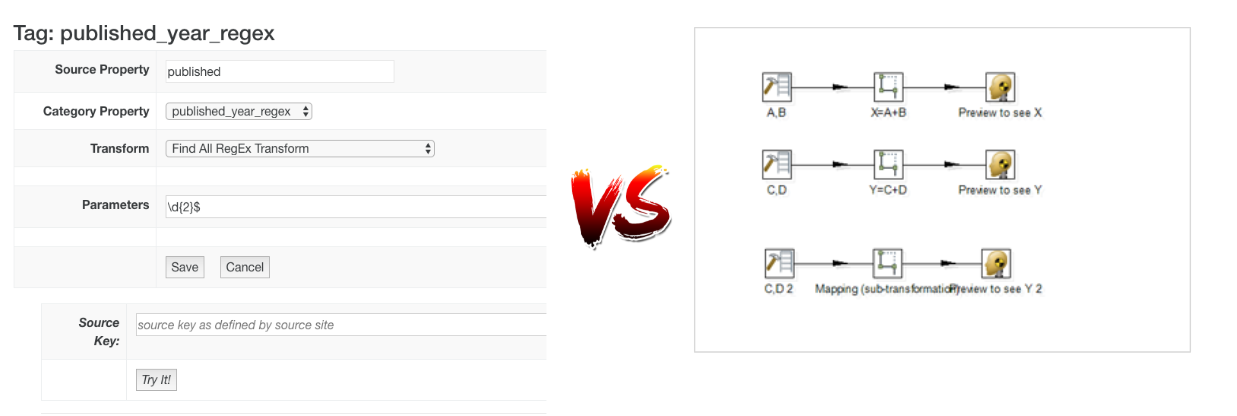
\includegraphics[scale=.35]{alternatives.png}
\caption{Transformation task for two interfaces: internal (left) and Pentaho Kettle (right)}
\label{fig::1}
\end{figure}

\subsection*{Data Inventory}
Selected approaches for needfinding - Participant, Interviews, and Analysis of existing interfaces - covered a large bulk of the Data Inventory. Interviews described currently known types of users based on their roles and expertise in interacting with the interface (\textbf{who are the users}). The Participant approach focused on the task itself, analyzing the steps requires to accomplish the goal (\textbf{what are their goals}, and \textbf{what are their tasks} and \textbf{subtasks}). Finally, with the Analysis of the Existing Interfaces from the perspective of hacks and workarounds, we gleaned into their needs - does the current interface include adequate capabilities to help the user in their goal (\textbf{what are their needs}). 

To complete the Data Inventory, we analyze the user's environment and look more thoroughly at the context in terms of the competing tasks.

\textbf{Where are the users} - The nature of the task - ETL - expects that users are either on their laptops, or desktops since they need access to a web browser, and sometimes a database. It is possible that some users may want to perform this task on mobile; however, it would be very cumbersome, and it is not anticipated that users would want to launch ETL-like processes from their phones. Therefore, our needfinding approaches have limited the user environment to desktops and laptops. 

\textbf{What is the context} During the interview process we have gathered information on the context, such as frequency and scale of interaction - how much data do users need to process, why they need to transform it, and how often do they have to repeat similar tasks. The nature of the interaction varied significantly by users roles. Users who were involved in prototyping new business use cases required efficiency for generating rules to mutate the data. Users who interacted with the external clients needed more visibility and ease of use. 

An interesting insight based on the observations for what else competes with user's attention relates to whether or not a user is required to be \textit{present} in the interface throughout the task. For example, when the user submits a new \textit{order} to transform a data field, they do not have to wait for the task to complete. Users may go and accomplish other tasks (check email, attend a meeting, have lunch, etc.) before returning to get the status of their first task. The phenomenon literally refers to the \textit{context switching} where the user can multitask to optimize their daily productivity. The ETL task should expect this behavior from the users, and provide information sufficient for the user to be able to pick up from where they left off. One such example is logging the most recent user's activity of the sidebar in the form of notifications. Another example is displaying the progress of the task being currently executed. In addition to bringing the user back to the context of task transformation, this feature provides a benefit of estimating time to completion. 


\subsection*{Defining Requirements}

Based on the results from the performed needfinding analysis, we can start describing the desired set of requirements for the interface that supports a data transformation task as part of the ETL process. The recommendations are provided for three areas - functionality, usability and learnability. Our analysis of existing users suggests that we need to cater to both, novices, and experts. The latter group benefits from the speed and efficiency, while the former is comforted with explorative feel of the interface.

\bigskip
\textbf{Functionality} - range of tasks supported for data transformation.

1) The interface must let user \textit{select} a source data intended for modification, \textit{choose} a transformation, \textit{save} the configuration and \textit{apply} the task to the dataset.

2) The interface should give the user a preview of the outcome for selected transformation \textit{before} the task is applied.

3) The interface should allow the user to create/edit/delete transformations, and optionally export it to a human-readable form.

\textbf{Usability} - quality of the available functionality.

1) The interface must support a transformation that is based on multiple sources, for example, combining two fields into one, or performing mathematical operations on them.

2) The interface must provide clear distinction between actions for \textit{saving} a configuration for a transformation, or \textit{applying} the transformation the data.

\textbf{Learnability} - ease and speed for the task of transforming data.

1) The interface should have a toolbox of standard transformations with meaningful names, and built-in tooltip that expands the capabilities of each transformation with examples.

2) The interface should provide clear messaging and notifications on the system's progress. For example, what is the most recent user's request, and what is its status.

3) The interface should allow the user to change the preferences on the order of the available transformations. The current order is alphabetical, and it does not help locate the needed transformation quickly. Options for ordering may include: 

\begin{itemize}
    \item Sort by relevance. Can the interface autodetect the transformations most compatible with the selected data type?
    \item Sort by recency. Show the transformations on top which were accessed last.
    \item Sort by popularity. A user may have a subset of transformations they access the most frequently, so it may be convenient to show a different set of transformations on top without requiring the user to scroll through the large list. 
\end{itemize}

Since the interface described in this project is an internal tool, I have access to the user's feedback that I could use to evaluate the successes of the prototype. For each of the items outlined, I am planning to gathers three data points: 1) priority 2) estimate for implementation 3) feasibility and alignment with the team's goals.  


\subsection*{Continuing Needfinding}
Conducting interviews gave me a wide range of perspectives on what and how the tool should accomplish the task. As a first step, this was very useful, and it steered my initial thoughts on the interface redesign in a different direction. I am planning to repeat the interviews by narrowing down the questions based on the outlined requirements. For the next iteration, the discussion may be focused on the following three areas:

1) What \textit{stylistic} improvements can be identified as low-hanging fruit in terms of implementation time, and value added to the user?

2) What \textit{existing} features require architectural discussions across teams, and how do they align with the customers' needs?

3) What \textit{new} features would give a strategic advantage for the current and upcoming use cases? 

In addition to narrowing down the scope of the question, I would also like to widen the user's roles that participated in the interviews. Specifically, a user in the Engineering role would likely be able to provide me with some rough estimates for UI and backend changes to support the redesign. Infrastructure-role users can be critical in addressing potential scale roadblocks. Also, finally, the CEO can provide guidelines on the strategy of execution. 

\bibliographystyle{apacite} 
\bibliography{bibtemp}

\section*{Appendices}

\appendix

\section{Interview Questions}

\subsubsection*{Section 1 - Data Presentation}
When deciding to transform a property, what is the value for you in being able to see the sample of existing data for the given property? If you do not see a value on that, please explain why.  If you see a value, please provide a recommendation on what constitutes a good sample, for example, you want to see the most recent values, the most frequent values, the most extreme values, etc. If you choose to say "yes" to the value, then please justify your needs. Here, you can describe your role, and why is this important to you.  

\subsubsection*{Section 2 - Data Transformation}
How frequently the data you loaded requires additional manipulation? What are your typical scenarios for transformations? When transforming a variable, do you need access to the other variables in a single record? What is one type of transformation that you need/want the most?  

\subsubsection*{Section 3 - Feedback/Recovery}
Do you feel that the current system's feedback is adequate? For example, recall scenarios where you wanted to transform a variable, but were struggling with the interface in terms of selecting needed information (selecting a transform type, configuring the transform, etc.). What is your experience at the times where the transformation you applied had an unexpected effect? Did you have enough information to understand the issue and/or recover your data and re-iterate the process?

\section{\\Interview Raw Responses}

\subsection*{Role: Senior Product Manager, Client Lead}
\subsubsection*{Question 1 - Data Presentation} 

\begin{itemize}
    \item I end up going through this process for at least half of our customers
    \item Data presentation is helpful, but only critical when a more complicated transformation is required (e.g., regex). Typically, I will look at the data PRIOR to this screen because I need to make the decision to do the transformation before I land here. 
    \item Once on this screen, it would be helpful to see the 'would be' output before it's changed.
    \item NOTE: this screen is currently just a config, not a processing screen. A more seamless flow would be very helpful!
\end{itemize}

\subsubsection*{Question 2 - Data Transformation}
\begin{itemize}
    \item I tend to think that an Excel/CSV/DB table format is the easiest way to look at this data (horizontally, one record per row). This is the way we load data into the system initially, too, so I'm already familiar with looking at data in this format. 
    \item Probably my most frequent transforms at this point are the concatenation (combining two or more values) or trimming/parsing/stripping from fields (e.g., removing characters)
    \item I don't do bucket transforms here, probably because I find them too difficult/not intuitive
    \item The dropdown has MANY transforms I have never used... largely because I don't know what they do. 
    \item The parameters field is applied inconsistently and isn't clear. What is supposed to go there? How do we configure these params? Better documentation needed.
    \item On my wishlist - it would be great to configure transcendence/standardization at this point too. Transcendence and tagging both feel like transforms to me.
\end{itemize}

\subsubsection*{Question 3 - Feedback/Recovery}
\begin{itemize}
    \item I think the issue here is two-fold. 1. This is just a configuration screen. It doesn't kick off any processing, so you could set this and never see the outcome. 2. We don't have an easy way to see the processed data until it is moved to the platform (aka production). Exposing these in a staging area would be ideal.
    \item There are additional steps required to get the data wired all the way through to 'final output' (e.g., the partner property). 
    \item Correcting errors is especially hard with our data processing tool. I believe we update a transform and reprocess to the correct values, but I'm not sure if that catches everything or if old/bad data can remain (e.g., if you mistakenly use a transform that in one case yields a value for a source entity... if you correct it, so now that new source entity has no value, does the old value go away?
\end{itemize}

\subsection*{Role: Chief Technical Officer}
\subsubsection*{Question 1 - Data Presentation}

\begin{itemize}
    \item Not using mental energy to imagine how data looks like before the transformation is very important to me; This allows to focus on the interface. Plus, imagination could be exhausting :)
\end{itemize}

\subsubsection*{Question 2 - Data Transformation}
\begin{itemize}
    \item I am involved in rapid prototyping for a variety of clients. During this phase, the data we get is very unclean; therefore I have to perform a lot of transformations.
    \item Main areas of transformations: Dictionary Mappings, Combining fields, Cleaning Up.
\end{itemize}

\subsubsection*{Question 3 - Feedback/Recovery}
\begin{itemize}
    \item \textit{Try it} functionality we currently have is a great way to provide feedback in the form of almost interactively reshaping the data
    \item An area where I stumble is around naming for the current transforms. A name is not always representative.
\end{itemize}

\subsection*{Role: Lead UX Designer}
\subsubsection*{Question 1 - Data Presentation}

\begin{itemize}
    \item It would be great to have a sneak peek into the data; however, one should be careful about not distracting the user from the task. Essentially, if the action of taking a look at the data underneath requires selecting multiple options, it does not improve the user's experience overall. 
\end{itemize}

\subsubsection*{Question 2 - Data Transformation}
\begin{itemize}
    \item Although, I am not currently using this feature, I can imagine a need for a transformation that requires multiple variables.
\end{itemize}

\subsubsection*{Question 3 - Feedback/Recovery}
\begin{itemize}
    \item The main advice in providing good feedback to the user is for the interface components to be consistent with the standard interfaces (buttons especially). For example, the actions should be ordered as \textit{Cancel}, \textit{Apply}, and \textit{Save}. In our case, \textit{Try it} button is below \textit{Save} which might confuse the user.
\end{itemize}

\subsection*{Role: Software Architect}

Note: For this interview, I did not have a chance to record the answers immediately, so I paraphrased their main takeaways
\subsubsection*{Question 1 - Data Presentation}

\begin{itemize}
    \item Although it is a noble goal to show the user a sample of the data, scalability of such requests needs to be considered carefully. Would this additional feature, although nice, interfere with the overall task.  
\end{itemize}

\subsubsection*{Question 2 - Data Transformation}
\begin{itemize}
    \item Too many transformations can be generalized and combined into a single function. No need to be too granular in what each function can do.  
\end{itemize}

\subsubsection*{Question 3 - Feedback/Recovery}
\begin{itemize}
    \item The users currently may suffer from system's frugal messaging when something goes wrong, and its verbosity for the typical workflow.
\end{itemize}

\end{document}
